\documentclass[12pt]{article}

%% Text-Encoding festlegen. Mit utf8 oder utf8x funktionieren Umlaute wie gewohnt.
%% (mit Bibtex funktioniert nur utf8)
\usepackage[utf8x]{inputenc}

%% Sprachdatei für Trennregeln, Datum-Format und ähnliches festlegen
\usepackage[german]{babel}  % nötig für Umlaute
% \usepackage[english]{babel}

%% optimiert das typographische Erscheinungsbild
\usepackage{microtype}

%% erlaubt Listen einfacher zu formatieren (bietet nosep für kompakte Listen)
\usepackage{enumitem}
%% erlaubt hübsche Tabellen über mehrere Seiten, beinhaltet booktabs (\toprule, \midrule, ...)
\usepackage{ctable}
%% ermöglicht farbigen Text ({\color{red} ...})
\usepackage{xcolor} 

%% erweiterte Funktionalität für Formeln (Pakete der American Mathematical Society)
\usepackage{amsfonts,amsmath,amsthm,amssymb}

%% vordefinierte Einheiten, einfaches Angeben von Einheiten (\SI{8 \pm 1}{cm})
%%   die Unsicherheit soll mit +- abgetrennt werden
\usepackage[separate-uncertainty]{siunitx}
\sisetup{
    range-units = single,       % \SIrange soll die Einheit nur einmal anzeigen
    list-units  = repeat,       % \SIlist soll die Einheit wiederholen
}
%% bei siuntix funktioniert babel leider nicht
%% für englische Dokumente sollten diese Zeilen auskommentiert werden. 
\sisetup{
    range-phrase         = { bis },
    list-final-separator = { und },
%    list-pair-separator  = { und }, % an Uni noch nicht verfügbar
}

%% erlaubt es Bilddateien einzubinden
%% (ctable graphicx intern auch. Trotzdem ist es sinnvoll graphicx expilizt zu laden.
%%  Sonst entstehen schwehr verständliche Fehler, wenn ctable entfernt wird)
\usepackage{graphicx}
%% ermöglicht Bilder und Tabellen am eingegebenen Ort zu platzieren ([H])
\usepackage{float}
%% ermöglicht Unter-Bilder in einer figure-Umgebung
\usepackage{subfig}
%% Grafik-Dateien werden in den folgenden Ordnern gesucht
\graphicspath{{img/}}
%% Grafikdateien haben die folgenden Endungen (höchste Priorität zu erst)
\DeclareGraphicsExtensions{.pdf,.png,.jpg}

%% Vertikaler Abstand zwischen Absätzen, Beginn eines Absatzes nicht einrücken
\usepackage{parskip}
% \setlength{\parskip}{0.6em}   % Vertikaler Abstand zwischen Absätzen anpassen 
% \setlength{\parindent}{0em}   % Einrück-Abstand anpassen 

%% zeige Labels im Seitenrand. Dies ist praktisch um Verweise zu kontrollieren
\usepackage[final]{showkeys} % die Option 'final' deaktiviert die Ausgabe von showkeys

%% Seiten-Layout einstellen
\usepackage[
 a4paper,
 total={18cm,28cm},          % Breite und Höhe des Inhalt-Bereichs
 top=10mm, left=12mm,        % Ränder oben und links
 headsep=0mm,               % Abstand des unteren Rands der Kopfzeile vom oberen Rand des Inhalts
 footskip=10mm               % Abstand des unteren des Inhalts zum oberen Rand der Fusszeile
]{geometry}

%% Ermöglicht Links im PDF 
%%   sollte möglichst spät in der Präambel geladen werden
\usepackage[
 pdftex,                        % wir verwenden pdftex/pdflatex
 bookmarks=true,                % wir wollen auch im PDF-Reader ein Inhaltsverzeichnis
 bookmarksdepth=3,              % das Inhaltsverzeichnis soll 3 Tiefen enthalten
 colorlinks=true,               % Linktexte sollen Farbig sein 
 linkcolor=black,               % Links innerhalb des Dokuments bleiben schwarz
 citecolor=black,               % Links zu Quellenangaben bleiben ebenfalls schwarz
 urlcolor=blue,                 % URL-Linktexte sollen blau dargestellt werden
%  pdfborder={0 0 0}              % Links im PDF erhalten keinen Rahmen, nur nötig wenn colorlinks=false
]{hyperref}

%% Angaben für die PDF-Eigenschaften
\hypersetup{
  pdfauthor = {Pascal Horat, Steve Gerome Kamga, G"okhan Kaya},
  pdftitle = {},
  pdfsubject = {},
  pdfkeywords = {}
}


%% definiert \cref: Referenzen mit korrekter Bezeichnung (z.B. "Abbildung 1")
%%   die Nummer alleine ist weiter mittels \ref verfügbar
%% muss NACH 'hyperref' geladen werden
\usepackage[german]{cleveref}
% \usepackage[english, capitalise]{cleveref}

\usepackage{tabulary}
\usepackage{array}

%% Angaben für \maketitle
\title{Reflexion Teamreview 1}
\author{Pascal Horat, Steve Gerome Kamga, Gökhan Kaya}
% \date{7. Mai 2013}             % ohne Angabe wird das heutig Datum verwendet

\begin{document}

\maketitle

\tableofcontents

\section{Zweck des Dokuments}

Dieses Dokuments hat zum Zweck das bisherige Arbeitsvorgehen sowie die ablaufenden Prozesse im Team zu dokumentieren und mit entsprechenden Literaturverweisen zu ergänzen. Daraus sollen wichtige Erkenntnisse bezüglich der Entwicklung unseres Teams gewonnen werden, welche uns in zukünftigen Teamarbeiten nützlich sein können.

\section{Bisheriges Vorgehen}

Da sich die Mitglieder unseres Teams gegenseitig noch nicht kannten, war unser erster Kontakt eine kurze informelle Vorstellungsrunde$^{[1]}$. Wir haben von Anfang an versucht, uns an die Abläufe und Dokumente welche in der Vorlesung behandelt wurden, sowie auf Moodle vorhanden sind, zu halten. Als Beispiel dafür könnte man das Verwenden von vorhandenen Vorlagen, anstatt diese selber zu verfassen, nennen. Daraus erhofften wir uns Leerläufe und Arbeiten welche nicht gefragt sind ersparen zu können. Dies gestaltete sich anfangs ziemlich schwierig, war die Plattform Moodle für einige unbekannt und beinhaltete eine Fülle von Dokumenten. Somit war der teamintern vereinbarte Auftrag der ersten Woche, sich einen Überblick über die vorhandenen Mittel auf Moodle zu verschaffen.

Der zweite grosse Schritt den das Team in Angriff genommen hat, war Abzuklären, was genau die von uns zu erledigenden Produkte$^{[2]}$ sind. Dies war uns auch nach Studieren der Moodle-Plattform noch nicht ganz klar. Darum erstellten wir zusammen einen Katalog mit Fragen, welche wir anschliessend dem Dozenten stellten. So konnte einiges geklärt werden.

Der nächste Schritt war das gemeinsame Ausarbeiten von Regeln, welche, sobald von allen Mitgliedern unterschrieben, für die Arbeit im Team verbindlich waren. Um dieses Regeldokument auszuarbeiten haben wir uns grob am GRPI Modell aus der Vorlesung$^{[3]}$ orientiert. Dabei sind wir folgendermassen vorgegangen:
\begin{enumerate}
\item Brainstorming\\
Das Team sass zusammen und Inputs der einzelnen Teammitglieder wurden, ohne diese zu werten, handschriftlich festgehalten.
\begin{center}
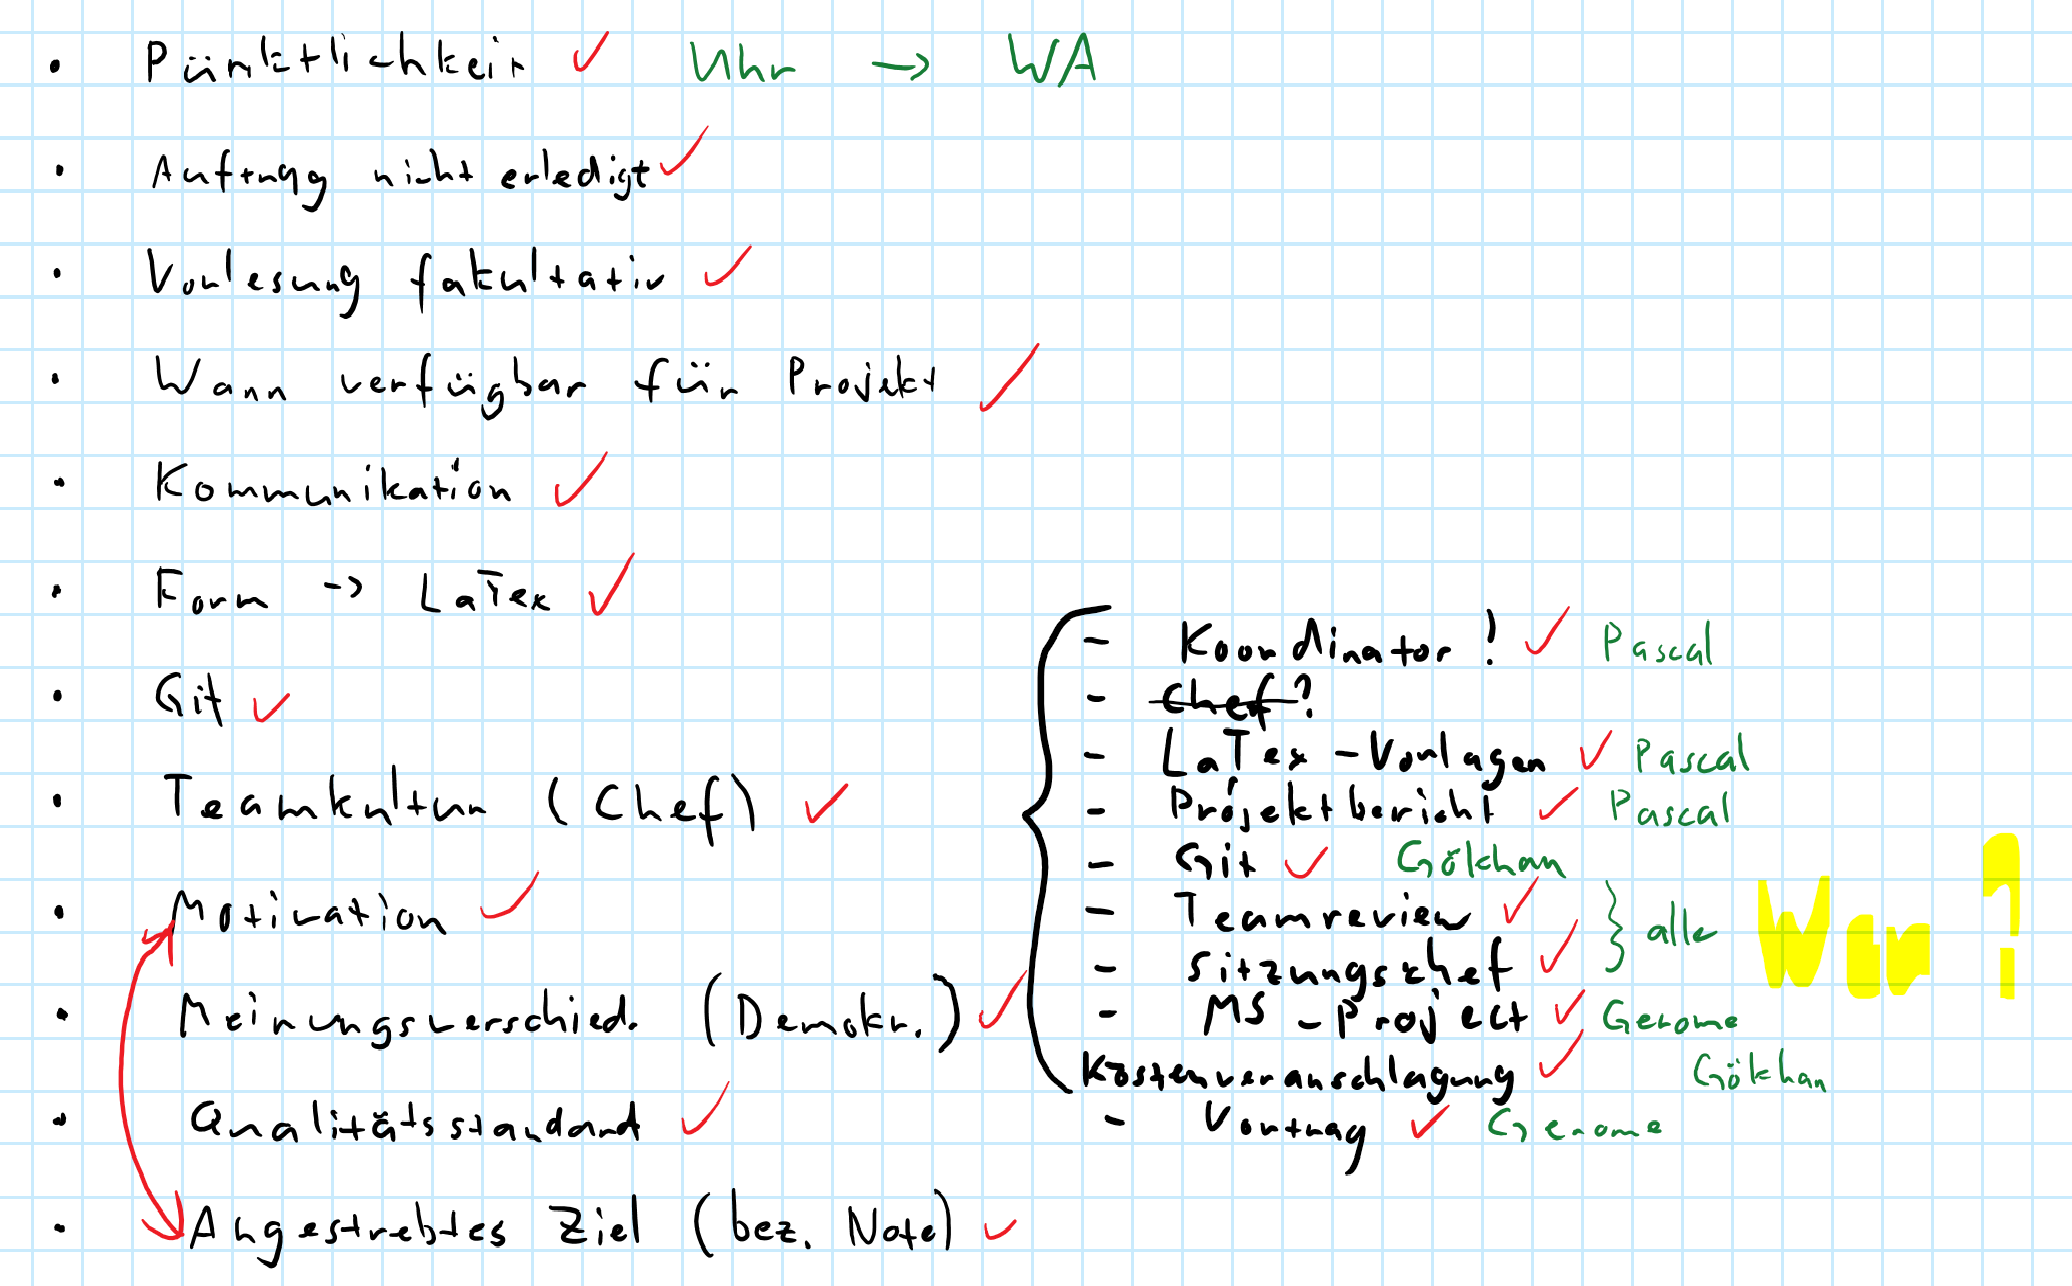
\includegraphics[scale=0.3]{regelnHand}
\end{center}
\item Sortierung\\
Um auf eine übersichtliche Anzahl Regeln zu kommen, wurden einzelne Punkte von uns zusammengenommen, andere komplett weggelassen.
\item Ausformulierung\\
Hier hat das Team im Plenum die gewählten Punkte zu Regeln ausformuliert und sich auf Konsequenzen bei Nichteinhalten geeinigt.
\item Erstellung Regeldokument\\
Schlussendlich wurden die formulierten Regeln in ein sauber formatiertes Dokument gepackt, welches der Übersicht halber mit je einem Bild pro Regel ergänzt wurde.
\item Anwendung\\
Da das Dokument von allen Mitgliedern unterschrieben worden ist, gelten nun diese Regeln für die zukünftige Arbeit in diesem Team.

\end{enumerate}


Die von uns in dem Regeldokument$^{[4]}$ gewählte Teamkultur, könnte am ehesten als die Ergebnisorientierte Kultur$^{[5]}$ beschrieben werden.



\section{Erkenntnisse}
\begin{itemize}
\item Obwohl unser Team zusammengestellt wurde, waren Probleme, auf die wir in diesen Phasen gestossen sind, eher externer als teaminterner Natur
\item In der Storming Phase$^{[6]}$ ist eine mögliche Rollenverteilung im Team relativ schnell ersichtlich
\item Obwohl wir uns im Regeldokument geeinigt haben, keinen eigentlichen Chef zu haben, ist der informelle Führer im Team einfach ausmachbar
\end{itemize}


 \section{Referenzen}
 
 
\begin{itemize}
\item[[1]] siehe Forming/Warming, Folie TE 1.1.6, S. 27 in TKI{\_}2017.02.20.1.pdf
\item[[2]] Folie PM	2.1.5/2.1.6, S. 37/38 in TKI{\_}2017.02.20.2.pdf
\item[[3]] Folie TE 1.1.2, S. 16 in TKI{\_}2017.02.20.1.pdf
\item[[4]] siehe TR1{\_}Elt1{\_}Regeldokument.pdf 
\item[[5]] Folie TE 2.1.1, S. 99 in TKI{\_}2017.02.27pdf
\item[[6]] siehe Storming, Folie TE 1.1.6, S. 27 in TKI{\_}2017.02.20.1.pdf
\end{itemize}
 
\end{document}
